%%%%%%%%%%%%%%%%%%%%%%%%%%%%%%%%%%%%%%%%%%%%%%%%%%%%%%%%%%%%%%%%%%
%%  ~ Trabajo de Fin de Grado - Universidad de Vigo (ESEI) ~    %%
%% Autor: Diego Enrique Fontán Lorenzo                          %%
%% Tutor: Miguel Ramón Díaz-Cacho Medina                        %%
%% Convocatoria: Julio 2020/21                                  %%
%% Título: Framework de automatización de auditorías Red Team   %%
%%%%%%%%%%%%%%%%%%%%%%%%%%%%%%%%%%%%%%%%%%%%%%%%%%%%%%%%%%%%%%%%%%

%%%%%%%%%%%%%%%%%%%%%%%%%%%%%
%% Software Design
%%%%%%%%%%%%%%%%%%%%%%%%%%%%%

\chapter{Diseño del \textit{software}} \label{cap:design}

En este capítulo se detallan los diferentes componentes de la aplicación (diseño estático) y cómo interactúan entre ellos (diseño dinámico).\n

%%%%%%%%%%%%%%%%%%%%%%%%%%%%%
%% Components diagram
%%%%%%%%%%%%%%%%%%%%%%%%%%%%%

\section{Diagrama de componentes} \label{sec:componentsdiagram}

Se han agrupado los componentes en dos paquetes principales \fig{componentsdiagram}: \textbf{\textit{User interface}}, relativo a los componentes diseñados mediante lenguajes de \textit{frontend}, y \textbf{\textit{Server}}, referente a aquellos procesos realizados en segundo plano y que tienen su base en lenguajes de \textit{backend}.\sn

\begin{figure}[H]
    \centering
    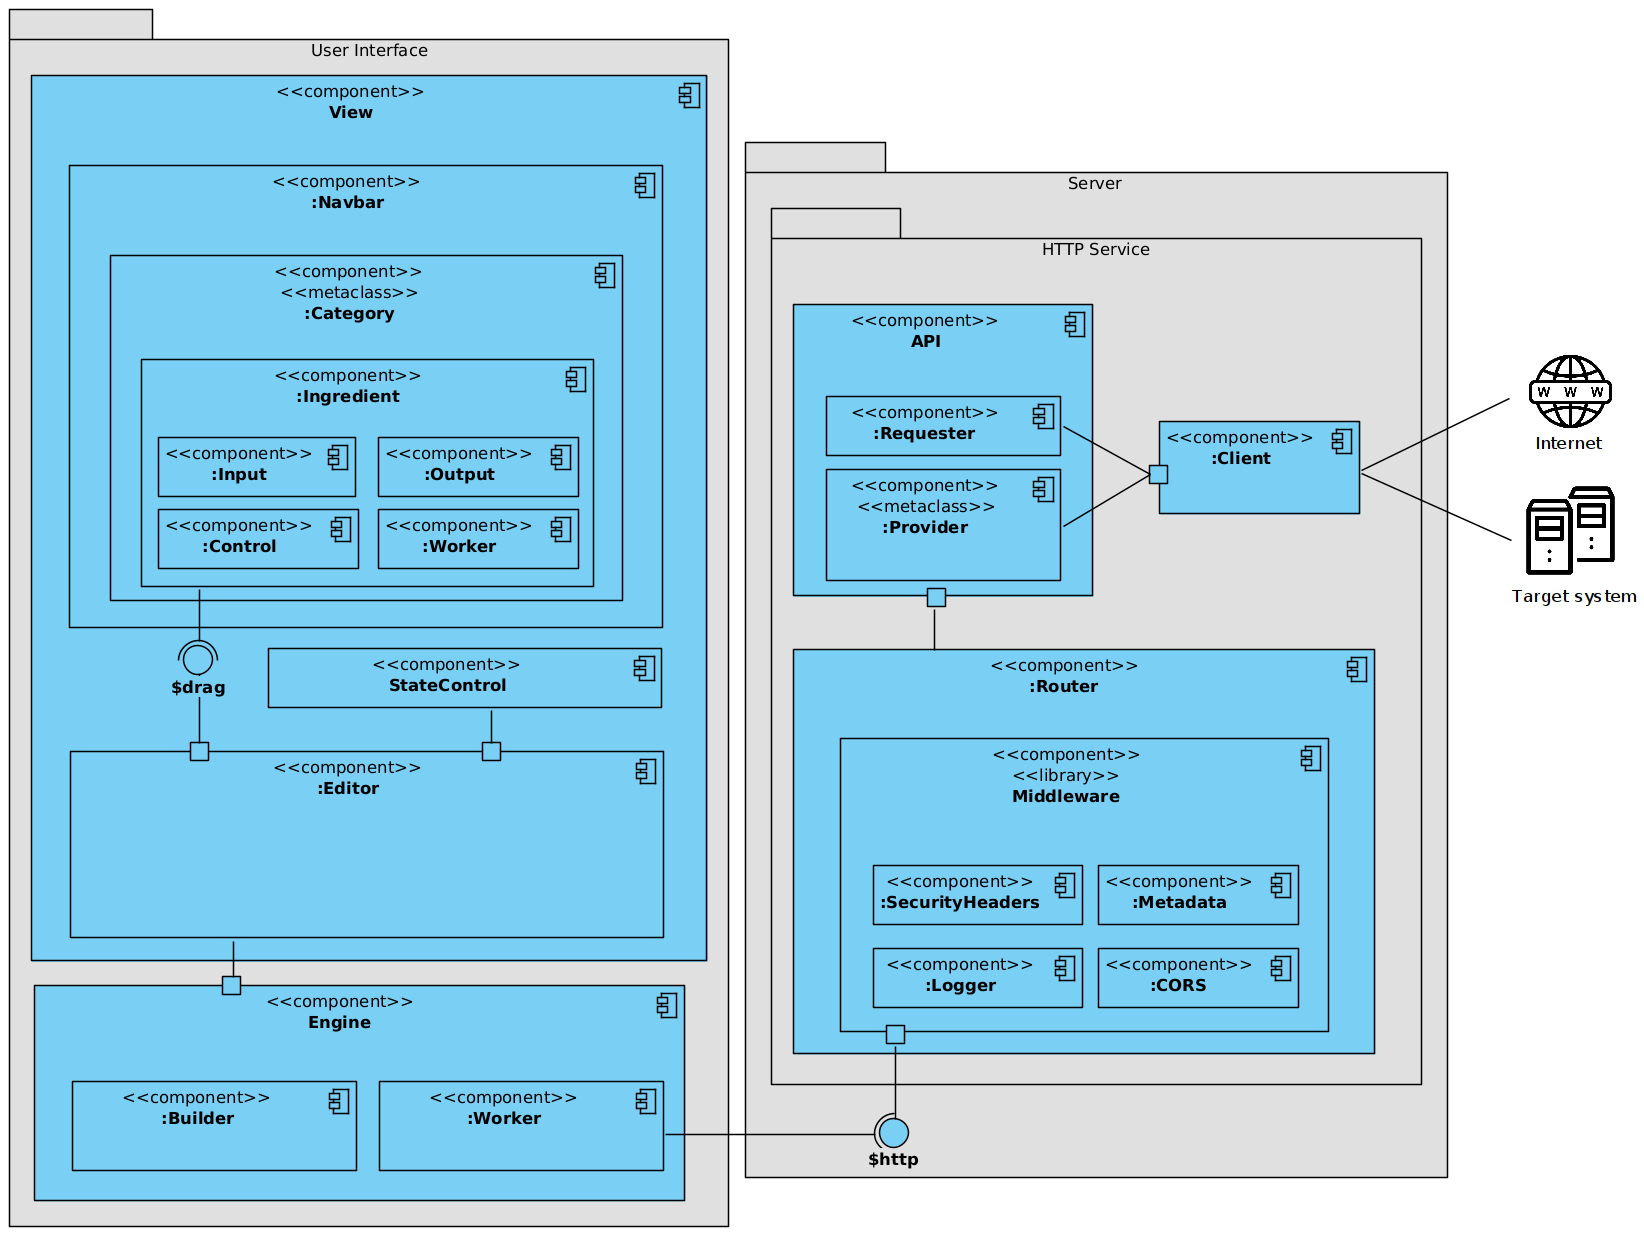
\includegraphics[width=15.5cm]{img/tables/19_Component-Diagram.png}
    \caption{Diagrama de componentes.}
    \label{fig:componentsdiagram}
\end{figure}

Se ha dividido a su vez el paquete \textit{Server}, creando una nueva agrupación llamada \textbf{\textit{HTTP Server}}, formado por los componentes que tienen relación con el procolo \textit{HTTP}. Esto tiene su origen en que no se descarta la idea de implementar nuevos servicios en un futuro (como \textit{FTP} o \textit{SMTP}).\sn

A continuación, se ofrece una pequeña descripción de la funcionalidad de cada componente.\n

Los componentes pertenecientes a la interfaz de usuario son:\sn

-- \textbf{View}: Encargado de renderizar la vista \textit{HTML} que compone la aplicación. Está formado, a su vez, por otras vistas.\sn

-- \textbf{Navbar}: Semi-vista del contenido lateral. Ofrece la opción de seleccionar y filtrar los \textit{Ingredients}.\sn

-- \textbf{Category}: Elemento contenedor de los diferentes \textit{Ingredients} agrupados según su funcionalidad.\sn

-- \textbf{Ingredient}: Uno de los dos elementos más importantes de la interfaz. Es la abstracción de cada una las tareas propias de una auditoría de ciberseguridad.

Está formado por componentes de entrada (o \textbf{\textit{Inputs}}), de salida (\textbf{\textit{Outputs}}), parámetros de configuración (\textbf{\textit{Controls}}) y un componente puramente funcional encargado de realizar las operaciones de cómputo (\textbf{\textit{Worker}}).\sn

-- \textbf{Editor}: El otro elemento más importante de la interfaz. Es el encargado de realizar las conexiones y renderizar los \textit{Ingredients} que lo forman\footnote{Para añadir un nuevo componente del tipo \textit{Ingredient} al \textit{Editor}, solamente basta con arrastrarlo. Los datos se transfieren a través del evento \textbf{\textit{drag}}.}.\sn

-- \textbf{StateControl}: Elemento encargado de manejar el estado general del \textit{Editor} mediante acciones de actualización, traslación, escalado, captura o carga.\sn

-- \textbf{Engine}: Se encarga de construir y registrar los \textit{Ingredientes} usando la especificación de la tarea correspondiente (\textbf{\textit{Builder}}).
También es el encargado de realizar las comprobaciones necesarias y manejar de forma asíncrona las tareas (\textbf{\textit{Worker}}).\n

Por otro lado, los componentes pertenecientes al servidor son:\sn

-- \textbf{Router}: Componente dedicado al enrutamiento de peticiones \textit{HTTP}.\sn

-- \textbf{API}: Componente encargado de realizar peticiones y procesar los datos relativos a servicios y sistemas externos.
Ofrece comunicación directa con los equipos auditados (\textbf{\textit{Requester}}) y obtención de información a través de fuentes abiertas (\textbf{\textit{Provider}}).\n

-- \textbf{Client}: Es el encargado de manejar las conexiones que requiere la \textit{API} y de definir las directrices por defecto de las peticiones.\sn

-- \textbf{Middleware}: Librería de componentes que tiene como objetivo modificar la respuesta \textit{HTTP} antes de que ésta sea servida.

Proporciona cabeceras de seguridad (\textbf{\textit{SecurityHeaders}}), de información (\textbf{\textit{Metadata}}), controla el intercambio de recursos de origen cruzado (\textbf{\textit{CORS}}) y registrar un seguimiento de las peticiones (\textbf{\textit{Logger}}).\sn


%%%%%%%%%%%%%%%%%%%%%%%%%%%%%
%% Packages diagram
%%%%%%%%%%%%%%%%%%%%%%%%%%%%%

\section{Diagrama de paquetes} \label{sec:packagesdiagram}

En esta sección se detalla la distribución por paquetes de la aplicación \fig{packagesdiagram}. En el caso concreto de la interfaz de usuario, dicha distribución se ha omitido debido a que todos los elementos están contenidos por un mismo paquete, el cual hace referencia a la única vista existente, que a su vez está formado por el resto de vistas parciales.\sn

Por otro lado, para lo referente al servidor, se ha seguido el modelo de paquetes que define \textit{Golang}\cite{gomod}, donde cada paquete o módulo no es más que un directorio que contiene una serie de archivos de código fuente. Además, tienen asociados las características relativas a un elemento o funcionalidad en concreto. Estos paquetes pueden, a su vez, contener otros paquetes. La dependencia entre uno o más módulos nunca puede ser cíclica.\sn

La distribución de paquetes es la siguiente:\sn

\begin{figure}[H]
    \centering
    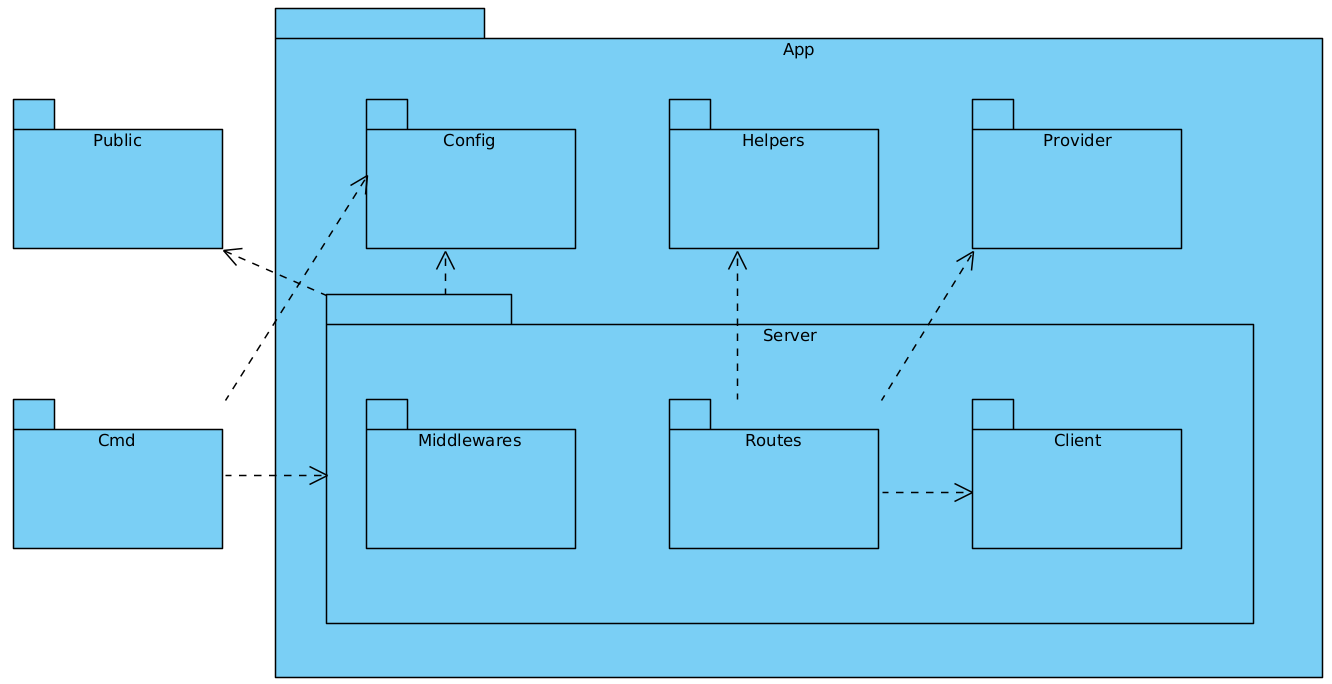
\includegraphics[width=15cm]{img/tables/20_Packages-Diagram.png}
    \caption{Diagrama de paquetes.}
    \label{fig:packagesdiagram}
\end{figure}
\newpage

Concretamente, cada paquete se puede definir como:\n

-- \textbf{Public}: Archivos estáticos propios de la interfaz gráfica.\sn

-- \textbf{Cmd}: Punto de entrada al ejecutar la aplicación.\sn

-- \textbf{App}: Núcleo del programa.\sn

-- \textbf{Config}: Parámetros de configuración necesarios para personalizar la ejecución.\sn

-- \textbf{Helpers}: Métodos auxiliares para el tratamiento de datos.\sn

-- \textbf{Provider}: Proveedores de información a través de fuentes abiertas.\sn

-- \textbf{Server}: Archivos relativos con el servidor \textit{HTTP} local. Contiene el enrutador.\sn

-- \textbf{Middlewares}: Acciones auxiliares para el procesamiento de peticiones \textit{HTTP}.\sn

-- \textbf{Routes}: Rutas estipuladas por el enrutador. Contiene los servicios de la \textit{API}.\sn

-- \textbf{Client}: Gestor de conexiones. Define las directrices por defecto de las peticiones.\n

%%%%%%%%%%%%%%%%%%%%%%%%%%%%%
%% Class diagram
%%%%%%%%%%%%%%%%%%%%%%%%%%%%%

\section{Diagrama de clases} \label{sec:classdiagram}

Una propiedad del modelo de paquetes que define \textit{Golang} \cite{gomod} (introducido en el apartado \ref{sec:packagesdiagram}) es la habilidad de cada paquete para ejercer como clase a pesar de no seguir un patrón relativo a la \textit{Programación Orientada a Objetos}. No existe el concepto de herencia y la visibilidad de los atributos y métodos se especifica capitalizando su nombre: si el identificador comienza por una letra mayúscula, la visibilidad es pública; en el caso contrario, es privada.\sn

El diagrama de clases correspondiente quedaría de la siguiente manera \fig{classdiagramserver}:\sn

\begin{figure}[H]
    \centering
    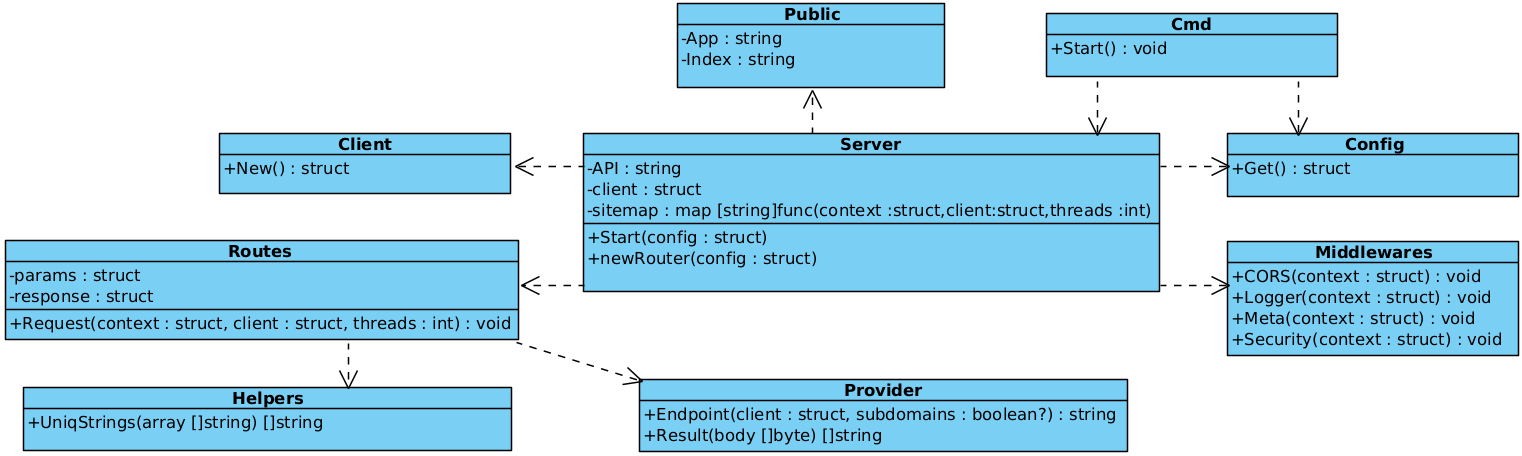
\includegraphics[width=15cm]{img/tables/21_Class-Diagram-Server.png}
    \caption{Diagrama de clases del servidor.}
    \label{fig:classdiagramserver}
\end{figure}
\newpage

Los atributos y métodos que aparecen en el diagrama son:\sn

\begin{table}[H]
    \begin{center}
        \begin{tabularx}{\textwidth}{| l | l | X |}
            \hline
            \multicolumn{3}{c}{ \textbf{Client} } \\ \hline
            \textbf{Propiedad} & \textbf{Nombre} & \textbf{Descripción} \\ \hline
            Método & New & Devuelve un nuevo cliente con los parámetros por defecto \\ \hline
        \end{tabularx}
    \end{center}
    \caption{Clase \textit{Client}.}
    \label{tab:classClient}
\end{table}

\begin{table}[H]
    \begin{center}
        \begin{tabularx}{\textwidth}{| l | l | X |}
            \hline
            \multicolumn{3}{c}{ \textbf{Cmd} } \\ \hline
            \textbf{Propiedad} & \textbf{Nombre} & \textbf{Descripción} \\ \hline
            Método & Start & Llama al servidor \textit{HTTP} usando la configuración dada\\ \hline
        \end{tabularx}
    \end{center}
    \caption{Clase \textit{Cmd}.}
    \label{tab:classCmd}
\end{table}

\begin{table}[H]
    \begin{center}
        \begin{tabularx}{\textwidth}{| l | l | X |}
            \hline
            \multicolumn{3}{c}{ \textbf{Config} } \\ \hline
            \textbf{Propiedad} & \textbf{Nombre} & \textbf{Descripción} \\ \hline
            Método & Get & Obtiene los parámetros de configuración \\ \hline
        \end{tabularx}
    \end{center}
    \caption{Clase \textit{Config}.}
    \label{tab:classConfig}
\end{table}

\begin{table}[H]
    \begin{center}
        \begin{tabularx}{\textwidth}{| l | l | X |}
            \hline
            \multicolumn{3}{c}{ \textbf{Helpers} } \\ \hline
            \textbf{Propiedad} & \textbf{Nombre} & \textbf{Descripción} \\ \hline
            Método & UniqString & Elimina los duplicados existentes en un \textit{array} de texto \\ \hline
        \end{tabularx}
    \end{center}
    \caption{Clase \textit{Helpers}.}
    \label{tab:classHelpers}
\end{table}

\begin{table}[H]
    \begin{center}
        \begin{tabularx}{\textwidth}{| l | l | X |}
            \hline
            \multicolumn{3}{c}{ \textbf{Middlewares} } \\ \hline
            \textbf{Propiedad} & \textbf{Nombre} & \textbf{Descripción} \\ \hline
            Método & CORS & Permite el intercambio de recursos de origen cruzado \\ \hline
            Método & Logger & Registra las peticiones \textit{HTTP} y sus respuestas \\ \hline
            Método & Meta & Añade cabeceras con \textit{metainformación} a las respuestas \\ \hline
            Método & Security & Añade cabeceras de seguridad a las respuestas \\ \hline
        \end{tabularx}
    \end{center}
    \caption{Clase \textit{Middlewares}.}
    \label{tab:classMiddlewares}
\end{table}
\newpage
\begin{table}[H]
    \begin{center}
        \begin{tabularx}{\textwidth}{| l | l | X |}
            \hline
            \multicolumn{3}{c}{ \textbf{Provider} } \\ \hline
            \textbf{Propiedad} & \textbf{Nombre} & \textbf{Descripción} \\ \hline
            Método & Endpoint & Devuelve la dirección de la fuente abierta \\ \hline
            Método & Result & Procesa la respuesta perteneciente a una fuente abierta \\ \hline
        \end{tabularx}
    \end{center}
    \caption{Clase \textit{Provider}.}
    \label{tab:classProvider}
\end{table}

\begin{table}[H]
    \begin{center}
        \begin{tabularx}{\textwidth}{| l | l | X |}
            \hline
            \multicolumn{3}{c}{ \textbf{Public} } \\ \hline
            \textbf{Propiedad} & \textbf{Nombre} & \textbf{Descripción} \\ \hline
            Atributo & App & Código \textit{JavaScript} relativo a la interfaz \\ \hline
            Atributo & Index & Plantilla \textit{HTML} relativa a la interfaz \\ \hline
        \end{tabularx}
    \end{center}
    \caption{Clase \textit{Public}.}
    \label{tab:classPublic}
\end{table}

\begin{table}[H]
    \begin{center}
        \begin{tabularx}{\textwidth}{| l | l | X |}
            \hline
            \multicolumn{3}{c}{ \textbf{Routes} } \\ \hline
            \textbf{Propiedad} & \textbf{Nombre} & \textbf{Descripción} \\ \hline
            Atributo & params & Parámetros \textit{HTTP} requeridos  \\ \hline
            Atributo & response & Parámetros \textit{HTTP} devueltos \\ \hline
            Método & Request & Realiza una petición \textit{HTTP} \\ \hline
        \end{tabularx}
    \end{center}
    \caption{Clase \textit{Routes}.}
    \label{tab:classRoutes}
\end{table}

\begin{table}[H]
    \begin{center}
        \begin{tabularx}{\textwidth}{| l | l | X |}
            \hline
            \multicolumn{3}{c}{ \textbf{Server} } \\ \hline
            \textbf{Propiedad} & \textbf{Nombre} & \textbf{Descripción} \\ \hline
            Atributo & API & Ruta y versión de la \textit{API} \\ \hline
            Atributo & client & Cliente \textit{HTTP} usado en las conexiones \\ \hline
            Atributo & sitemap & Parejas de rutas y servicios de la \textit{API} \\ \hline
            Método & Start & Levanta el servidor \textit{HTTP} usando la configuración dada \\ \hline
            Método & newRouter & Devuelve un nuevo enrutador \\ \hline
        \end{tabularx}
    \end{center}
    \caption{Clase \textit{Server}.}
    \label{tab:classServer}
\end{table}

Cabe destacar que tanto \textit{Provider} como \textit{Routes} se tratan de \textit{super clases}, similares a una interfaz, que especifican los métodos y atributos propios de sus clases derivadas. Su diseño se debe a la futura creación y soporte de \textit{plugins}.\n

\newpage
Por otro lado, para el desarrollo de la interfaz también se ha usado un formato basado en clases que se puede representar mediante el siguiente diagrama \fig{interfaceclassdiagram}:\sn

\begin{figure}[H]
    \centering
    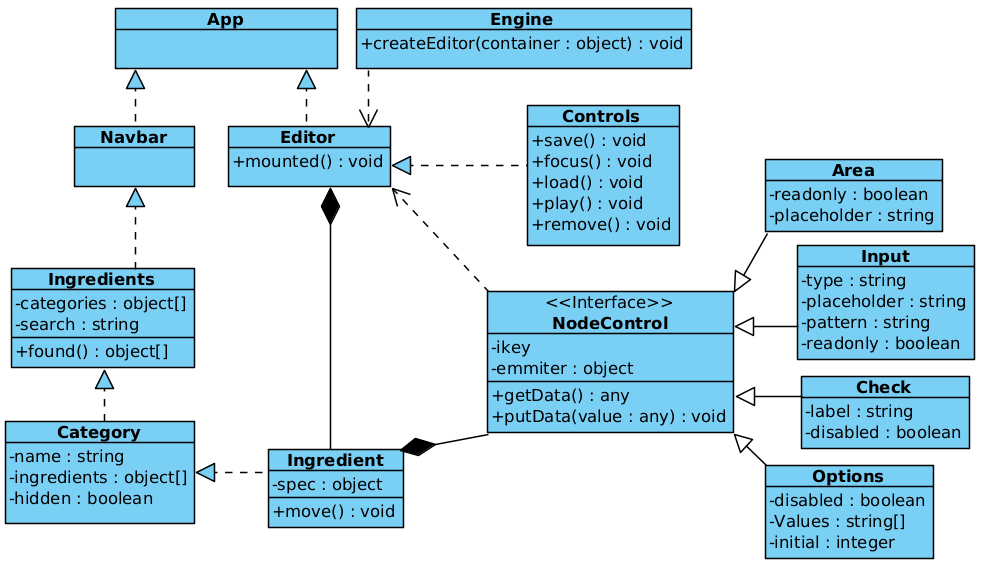
\includegraphics[width=15cm]{img/tables/22_Class-Diagram-UserInterface.png}
    \caption{Diagrama de clases de la interfaz.}
    \label{fig:interfaceclassdiagram}
\end{figure}

Los atributos y métodos que aparecen en el diagrama son:\sn

\begin{table}[H]
    \begin{center}
        \begin{tabularx}{\textwidth}{| l | l | X |}
            \hline
            \multicolumn{3}{c}{ \textbf{Engine} } \\ \hline
            \textbf{Propiedad} & \textbf{Nombre} & \textbf{Descripción} \\ \hline
            Método & createEditor & Crea, inicializa y agrega el editor a la estructura \textit{HTML} \\ \hline
        \end{tabularx}
    \end{center}
    \caption{Clase \textit{Engine}.}
    \label{tab:classEngine}
\end{table}

\begin{table}[H]
    \begin{center}
        \begin{tabularx}{\textwidth}{| l | l | X |}
            \hline
            \multicolumn{3}{c}{ \textbf{Editor} } \\ \hline
            \textbf{Propiedad} & \textbf{Nombre} & \textbf{Descripción} \\ \hline
            Método & mount & Evento realizado tras montar la vista en la aplicación \\ \hline
        \end{tabularx}
    \end{center}
    \caption{Clase \textit{Editor}.}
    \label{tab:classEditor}
\end{table}

\begin{table}[H]
    \begin{center}
        \begin{tabularx}{\textwidth}{| l | l | X |}
            \hline
            \multicolumn{3}{c}{ \textbf{Ingredients} } \\ \hline
            \textbf{Propiedad} & \textbf{Nombre} & \textbf{Descripción} \\ \hline
            Atributo & categories & Categorias relativas a los ingredientes \\ \hline
            Atributo & search & Término usado durante la búsqueda de ingredientes \\ \hline
            Método & found & Ingredientes filtrados durante la búsqueda \\ \hline
        \end{tabularx}
    \end{center}
    \caption{Clase \textit{Ingredients}.}
    \label{tab:classIngredients}
\end{table}

\begin{table}[H]
    \begin{center}
        \begin{tabularx}{\textwidth}{| l | l | X |}
            \hline
            \multicolumn{3}{c}{ \textbf{Category} } \\ \hline
            \textbf{Propiedad} & \textbf{Nombre} & \textbf{Descripción} \\ \hline
            Atributo & name & Nombre de la categoría \\ \hline
            Atributo & ingredients & Ingredientes pertenecientes a la categoría \\ \hline
            Método & hidden & Define el estado relativo a su visualización \\ \hline
        \end{tabularx}
    \end{center}
    \caption{Clase \textit{Category}.}
    \label{tab:classCategory}
\end{table}

\begin{table}[H]
    \begin{center}
        \begin{tabularx}{\textwidth}{| l | l | X |}
            \hline
            \multicolumn{3}{c}{ \textbf{Ingredient} } \\ \hline
            \textbf{Propiedad} & \textbf{Nombre} & \textbf{Descripción} \\ \hline
            Atributo & spec & Nombre de la categoría \\ \hline
            Método & move & Genera la información requerida por el evento \textit{drag}  \\ \hline
        \end{tabularx}
    \end{center}
    \caption{Clase \textit{Ingredient}.}
    \label{tab:classIngredient}
\end{table}

\begin{table}[H]
    \begin{center}
        \begin{tabularx}{\textwidth}{| l | l | X |}
            \hline
            \multicolumn{3}{c}{ \textbf{Controls} } \\ \hline
            \textbf{Propiedad} & \textbf{Nombre} & \textbf{Descripción} \\ \hline
            Método & save & Guarda el estado actual del editor en un archivo \textit{.recipe} \\ \hline
            Método & focus & Hace zoom en los nodos del editor \\ \hline
            Método & load & Carga el estado del editor a través de un archivo \textit{.recipe} \\ \hline
            Método & play & Inicia el flujo de datos \\ \hline
            Método & remove & Limpia el editor de nodos \\ \hline
        \end{tabularx}
    \end{center}
    \caption{Clase \textit{Controls}.}
    \label{tab:classControls}
\end{table}

\begin{table}[H]
    \begin{center}
        \begin{tabularx}{\textwidth}{| l | l | X |}
            \hline
            \multicolumn{3}{c}{ \textbf{NodeControl} } \\ \hline
            \textbf{Propiedad} & \textbf{Nombre} & \textbf{Descripción} \\ \hline
            Atributo & ikey & Identificador del control \\ \hline
            Atributo & emitter & Gestor de eventos \\ \hline
            Método & getData & Obtiene el valor del estado interno \\ \hline
            Método & putData & Cambia el valor del estado interno \\ \hline
        \end{tabularx}
    \end{center}
    \caption{Clase \textit{NodeControl}.}
    \label{tab:classNodeControl}
\end{table}

%%%%%%%%%%%%%%%%%%%%%%%%%%%%%
%% Sequence diagram
%%%%%%%%%%%%%%%%%%%%%%%%%%%%%

\section{Diagramas de secuencia} \label{sec:sequencediagram}

Las interacciones entre las diferentes clases se entiende mejor al esquematizarlas mediante diagramas dinámicos, como el diagrama de secuencias. Por otra parte, la ejecución de un conjunto de tareas mediante el uso de la aplicación, como puede ser una auditoría de seguridad, ya es en sí mismo un diagrama de flujo, por la naturaleza propia de un editor gráfico basado en nodos.\sn

\newpage

La figura \ref{fig:seqdiagraminterface} muestra el flujo de datos al hacer \textit{click} sobre el botón de ejecución. El editor manda el evento al motor, el cual es el encargado de llamar a todos los nodos por orden. Los nodos, a su vez, tienen la capacidad de obtener del editor el estado de los datos y, si es preciso, hacer llamadas al servidor para que interactuar con servicios externos. Después de calcular el resultado en función de los parámetros obtenidos, comunica su respuesta y emite una señal al motor para que se ejecuten los siguientes nodos. Esta tarea finaliza cuando todos los nodos han sido procesados.\sn

\begin{figure}[H]
    \centering
    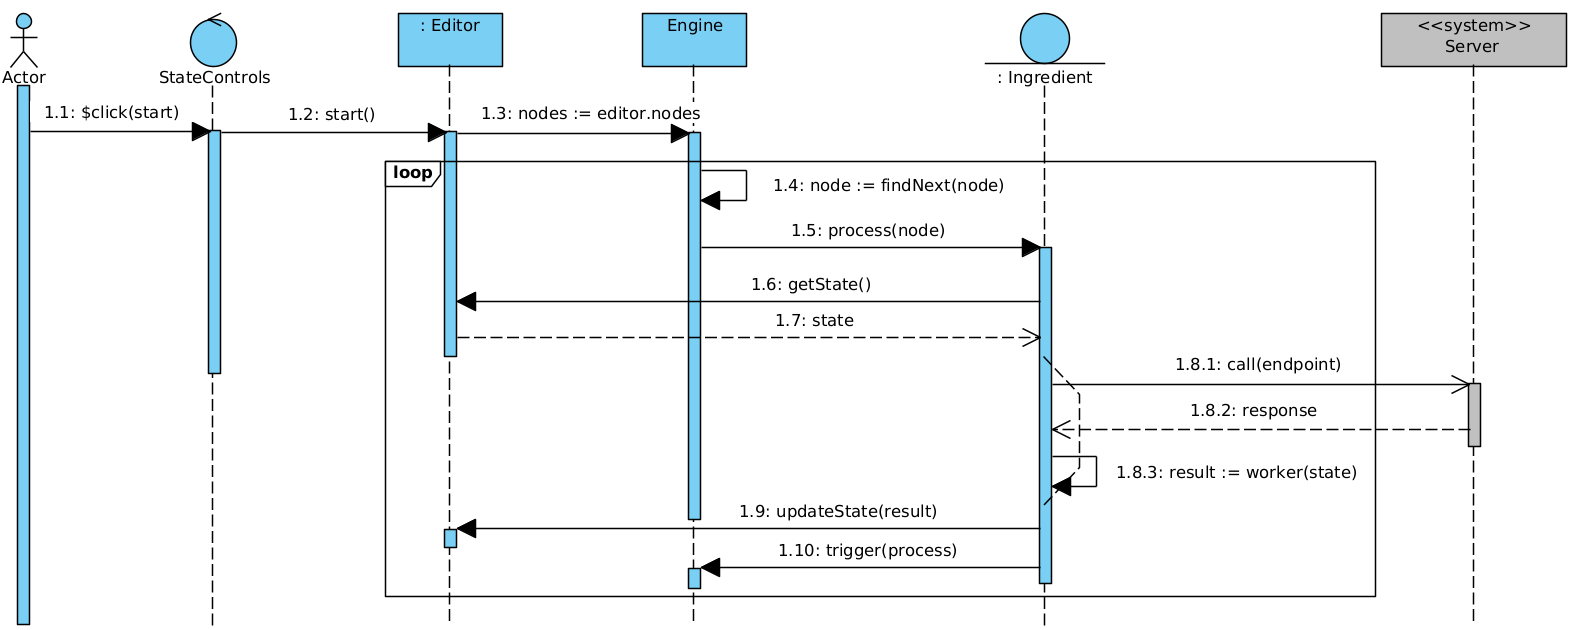
\includegraphics[width=15cm]{img/tables/23_Sequence-Diagram-Interface.png}
    \caption{Diagrama de secuencia de la interfaz.}
    \label{fig:seqdiagraminterface}
\end{figure}

Por otra parte, cuando se hace una llamada al servidor \fig{seqdiagramserver}, el enrutador comprueba que la petición esté correctamente formada. Después, pasa el contexto de la petición a los \textit{middlewares} para que se encarguen de aplicar las cabeceras necesarias (de seguridad, de información y de intercambio de recursos). Una vez el contexto vuelve a estar en manos del enrutador, comprueba la petición y la manda al \textit{Requester} (si se necesita interactuar directamente con el objetivo) o a uno de los \textit{Providers} (si se requiere de información disponible en fuentes abiertas\footnote{Las fuentes abiertas muchas veces contienen datos duplicados, por lo que se ha de limpiar la respuesta}). Antes de que la respuesta llege de nuevo al enrutador, el \textit{middleware} de \textit{logging} registra la petición junto al estado de la respuesta. Por último, se devuelve la respuesta al nodo que la pidió.\sn

\begin{figure}[H]
    \centering
    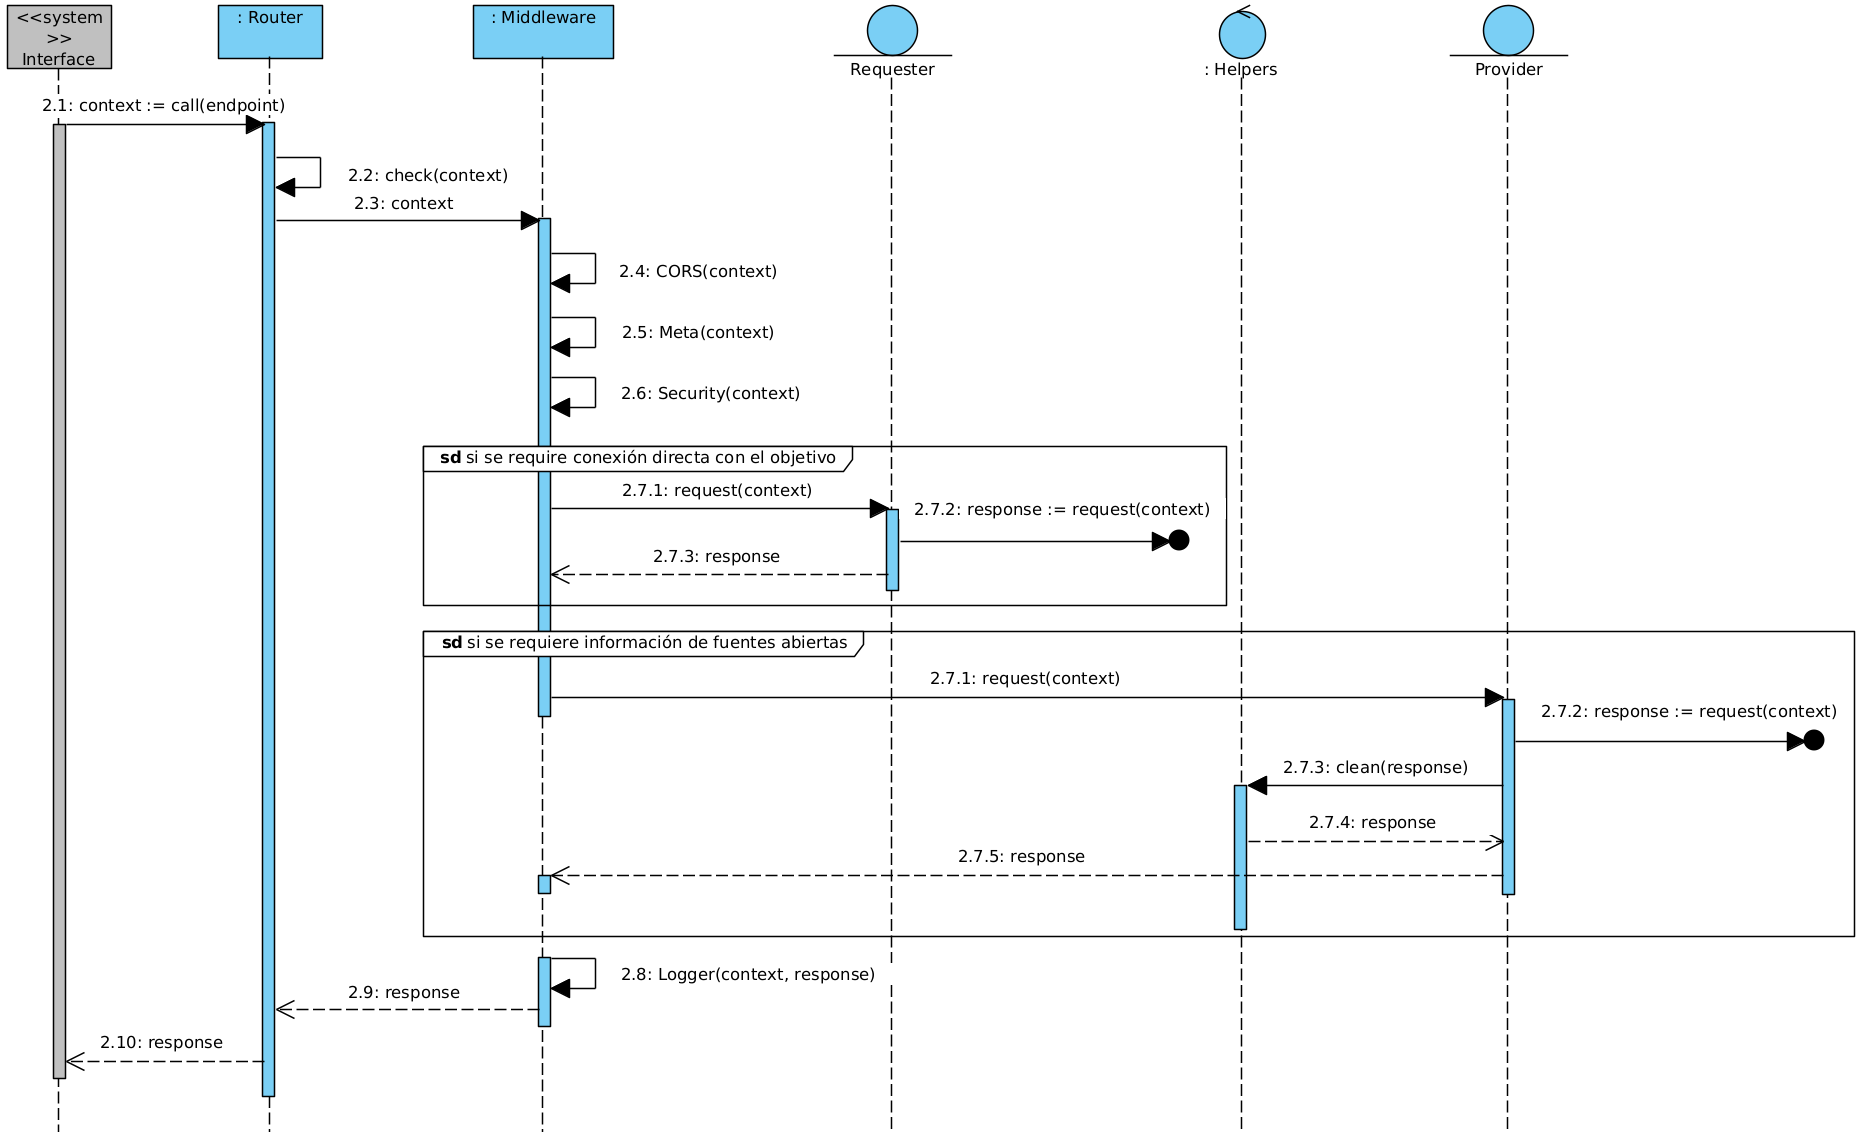
\includegraphics[width=15cm]{img/tables/24_Sequence-Diagram-Server.png}
    \caption{Diagrama de secuencia del servidor.}
    \label{fig:seqdiagramserver}
\end{figure}

%%%%%%%%%%%%%%%%%%%%%%%%%%%%%
%% Interface design
%%%%%%%%%%%%%%%%%%%%%%%%%%%%%

\section{Diseño de la interfaz gráfica} \label{sec:graphicinterface}

A continuación, se muestra un boceto de la interfaz \fig{userinterface}, que constará de una única página dinámica. Contiene un \textit{banner} con el nombre de la aplicación, el editor (controlado por botones en la parte inferior de la interfaz) y una barra lateral con un buscador y los diferentes nodos agrupados por categorías.\sn

Los nodos podrán añadirse al editor e interconectarse entre sí por medio del evento \textit{drag} (arrastrando el cursor mientras se presiona).\sn

\begin{figure}[H]
    \centering
    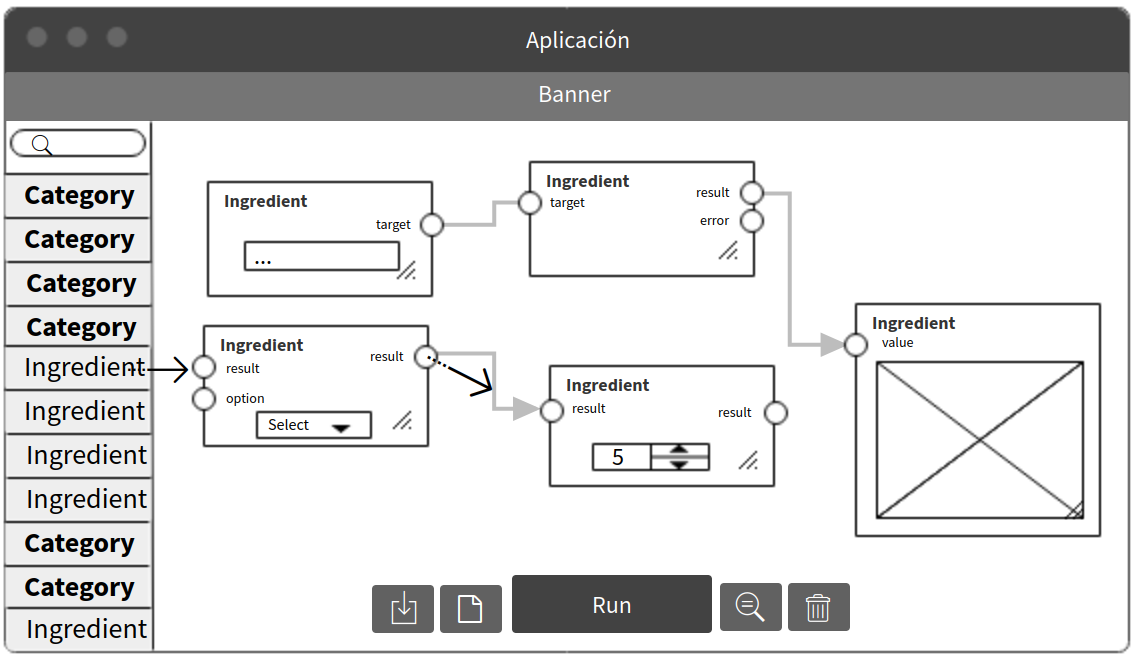
\includegraphics[width=12cm]{img/tables/25_User-Iterface.png}
    \caption{Diseño de la interfaz de usuario.}
    \label{fig:userinterface}
\end{figure}